%!TEX root = main.tex
\section{Modelling}
This report will analyze how a virus outbreak evolves over time on a global scale. To do so, firstly it will be described how one might model a virus outbreak in a small uniform population. Secondly, this model will be expanded to include multiple population groups and their interactions.

\subsection{The SIR Model}
\subsubsection{Assumption}
The Susceptible-Infected-Removed model is a compartmental model assuming that within some subdivision of the population containing $N$ individuals, infection rate, cure rate and spread rates are i.i.d.\todo{i.i.d. infer some distribution, but this is a deterministic model.} within each of the 3 ``compartments'' of individuals:
\begin{itemize}
	\item Susceptible to the virus
	\item Infected by the virus
	\item Recovered and immune to the virus (or alternatively dead)
\end{itemize} 
In reality economic status, job type, air-conditioning etc. will affect how a virus spread \cite{zika-modelling}, however, depending on the heterogeneity of the population these assumptions constitute a good approximation.

\subsubsection{Governing equations}
The SIR model is governed by 3 differential equations \cite{sir-basics}:
\begin{align}
\frac{d S(t)}{dt} &= - \beta \frac{I(t)}{N} S(t)   \label{eq-S}\\
\frac{d I(t)}{dt} &= \beta \frac{I(t)}{N} S(t) - \gamma I(t)  \label{eq-I}\\
\frac{d R(t)}{dt} &= \gamma I(t) \label{eq-R}
\end{align}
$S(t), I(t)$ and $R(t)$ are functions describing the number of susceptible, infected and removed (recovered and immune or dead) individuals at time t, $\beta$ is the rate of infection, $\gamma$ the rate of removal (dead or cured) and $N$ the total number of individuals.

From equation \eqref{eq-S} and \eqref{eq-I} one can see that susceptible individuals become infected by some ratio $\beta$ and the ratio of already infected individuals. From \eqref{eq-I} and \eqref{eq-R} one can see that infected individuals recover with a constant factor $\gamma$. 

\begin{figure}[H]
	\centering
	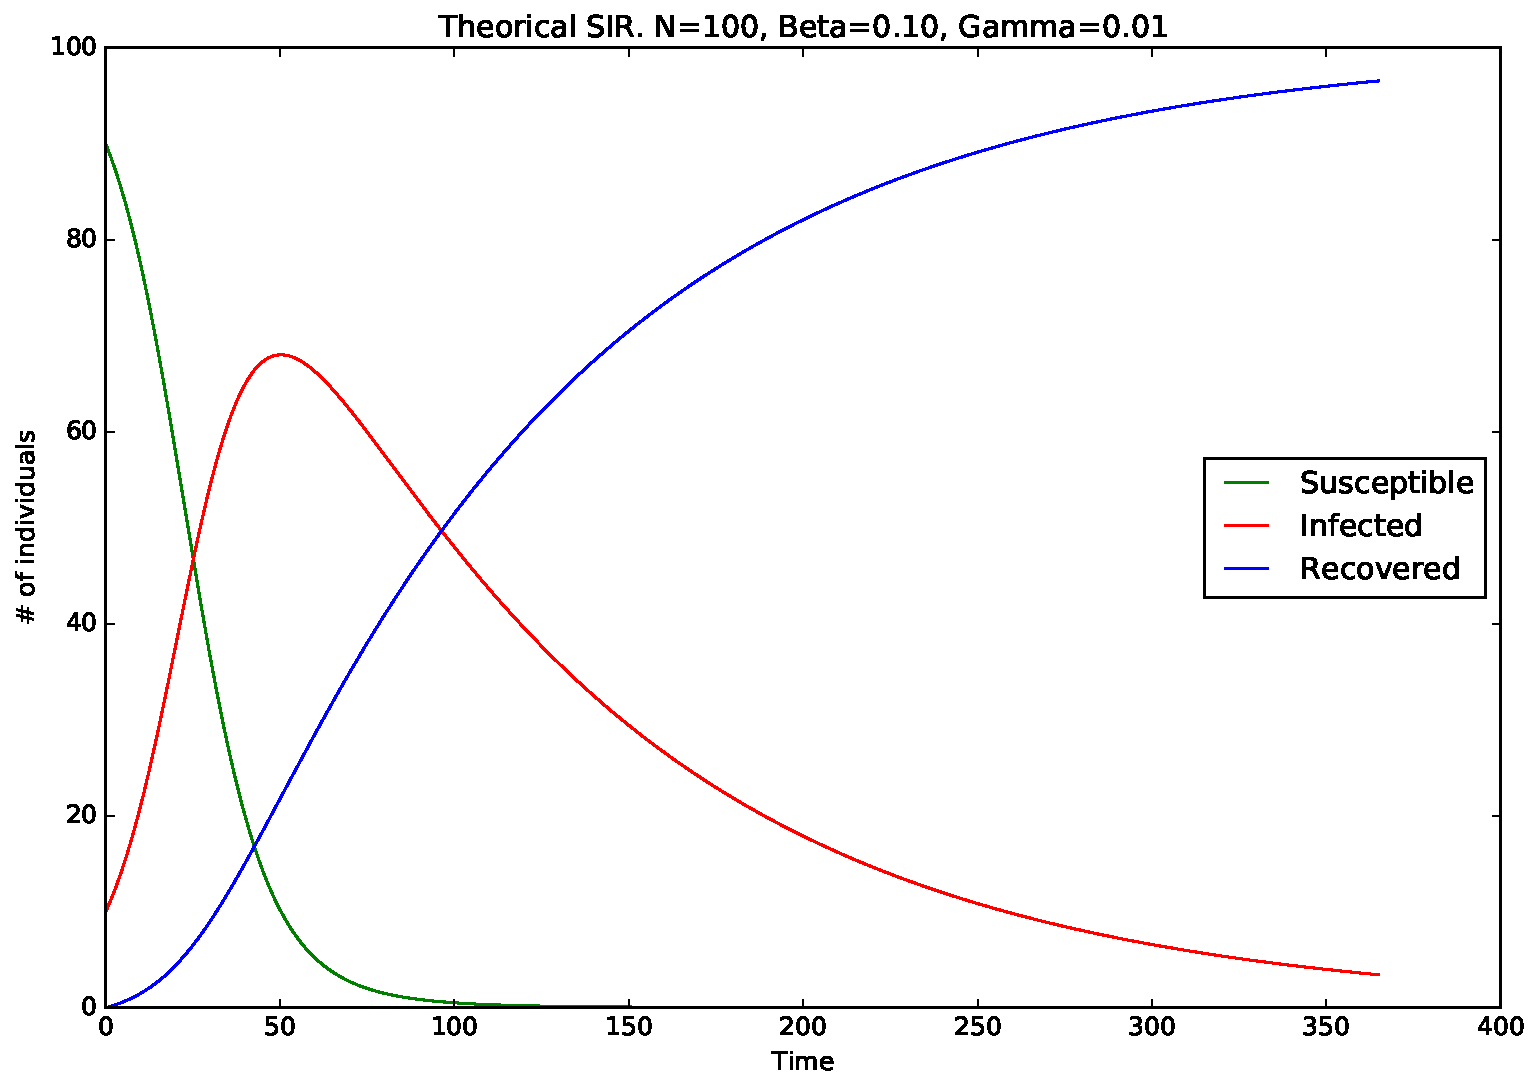
\includegraphics[width= 1.0 \linewidth]{plots/sir_one_region.pdf}
	\caption{Numerical solution to the nonlinear ODE system defining the SIR model.}
	\label{fig:sir_one_region}
\end{figure}

From figure \ref{fig:sir_one_region} it seen how the number of infected individuals increases quickly in the beginning, until a point where there are not enough susceptible to sustain the infection rate. This is also seen from the differential equations:
\begin{equation}
\frac{d I(t)}{dt} = \frac{\beta}{N} I(t) S(t) - \gamma I(t) = 0 \Leftrightarrow \beta\frac{S(t)}{N} = \gamma
\end{equation}

In this hypothetical case almost everybody got infected, but that is not necessarily the case and depends entirely on $\gamma$ and $\beta$.

\subsection{Multi-region SIR}
Let it now be given that instead of having a single population, one has $K$ populations each with initial $N_k, S_k(0), I_k(0)$ and $R_k(0)$. Each of these populations have a probability of transferring individuals to other populations regardless of whether the individual is susceptible, infected or recovered. The governing equations are modified to add the transfers and become
\begin{equation}
\begin{aligned}
\frac{d S_k(t)}{dt} &= - \frac{\beta}{N_k} I(t) S(t) + \sum_{i=1}^K \left( S_i(t)\tau_{i,k} - S_k(t)\tau_{k, i}\right)   &\forall k \in [1, K]\\
\frac{d I_k(t)}{dt} &= \frac{\beta}{N_k} I(t) S(t) - \gamma I(t) + \sum_{i=1}^K \left( I_i(t)\tau_{i,k} - I_k(t)\tau_{k, i}\right)  &\forall k \in [1, K]\\
\frac{d R_k(t)}{dt} &= \gamma I(t) + \sum_{i = 1}^K \left( R_i(t)\tau_{i,k} - R_k(t)\tau_{k, i}\right) &\forall k \in [1, K]
\end{aligned}
\end{equation}
, where $\tau_{i,j}$ is the probability density of transferring from population $i$ to $j$ per individual.

As an example of the above system let $K=3$ and the non zero transfer probabilities be defined by the graph:
\begin{figure}[H]
	\centering
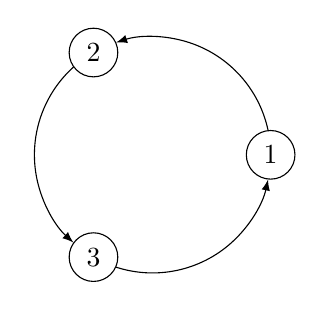
\begin{tikzpicture}

\def \n {3}
\def \radius {1.5cm}
\def \margin {12} % margin in angles, depends on the radius

\foreach \s in {1,...,\n}
{
	\node[draw, circle] at ({360/\n * (\s - 1)}:\radius) {$\s$};
	\draw[->, >=latex] ({360/\n * (\s - 1)+\margin}:\radius) 
	arc ({360/\n * (\s - 1)+\margin}:{360/\n * (\s)-\margin}:\radius);
}
\end{tikzpicture}
\end{figure}
Solving this system numerically with the outbreak starting in region 1 one yields the following curves:
\begin{figure}[H]
	\centering
	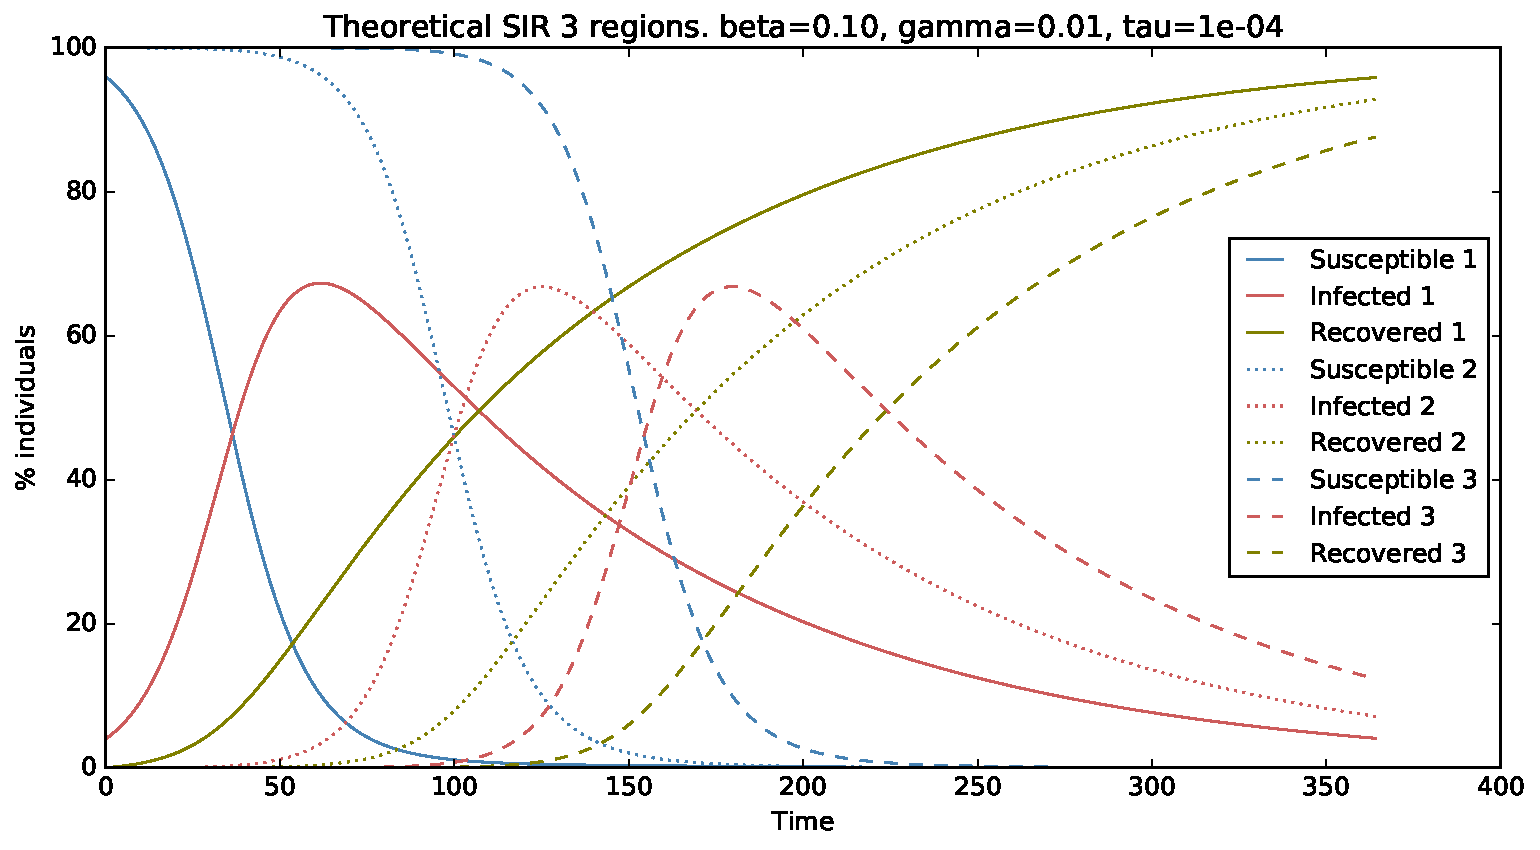
\includegraphics[width= 1.0 \linewidth]{plots/sir_three_region_theory.pdf}
	\caption{Numerical solution of the nonlinear ODE system defining a 3-region SIR model.}
\end{figure}

From the above plot it's seen that the virus first spreads in region 1. After a certain time enough infected individuals have been transferred to region 2 where the infection then accelerates. This continues to region 3.

\subsection{Stocastic Model}

To simulate the multi-region SIR model stochastically, a binomial distribution is used to sample how many people get infected, removed and transferred. The binomial probability is chosen such that the distribution's expectation is the same as the terms in the differential equations,
\begin{equation*}
\begin{aligned}
\Delta I_{k,t} &= \textsc{Binom}\left(S_{k,t}, \beta \frac{I_{k, t}}{N_k}\right) \\
\Delta R_{k,t} &= \textsc{Binom}\left(I_{k,t}, \gamma\right) \\
S_{k,t} &= S_{k,t-1} - \Delta I_{k,t} + \sum_{i = 1}^K \left(\textsc{Binom}(S_{i,t-1}, \tau_{i,k}) - \textsc{Binom}(S_{k,t-1}, \tau_{k,i})\right) \\
I_{k,t} &= I_{k,t-1} + \Delta I_{k,t} - \Delta R_{k, t} + \sum_{i = 1}^K \left(\textsc{Binom}(I_{i,t-1}, \tau_{i,k}) - \textsc{Binom}(I_{k,t-1}, \tau_{k,i})\right) \\
R_{k,t} &= R_{k,t-1} + \Delta R_{k, t} + \sum_{i = 1}^K \left(\textsc{Binom}(R_{i,t-1}, \tau_{i,k}) - \textsc{Binom}(R_{k,t-1}, \tau_{k,i})\right)
\end{aligned}
\end{equation*}

, where $\tau_{i,j}$ now is the discretized transfer probability.

\subsubsection{Transfer using Dirichlet distribution}
A problem with this approach, is the small risk that $\textsc{Binom}(S_{i, t-1}, \tau_{i,k}) = 0$ and $\textsc{Binom}(S_{k, t-1}, \tau_{k,i}) = S_k$ or similar unfortunate combination which would cause $S_{k,t}$ to become negative (i.e. there is a small non zero probability that if transfers are drawn independently that an unfeasible state would occur). In practice, this is a big problem if the number of regions is large. The only way to avoid this problem is to sample all the transfers for a region simultaneously such that $\sum_{i = 1}^K \textsc{Binom}(S_{k,t-1}, \tau_{k,i}) \le S_{k, t}$.

As there does not exist a multivariate version of the binomial distribution, the Dirichlet distribution is used as an approximation. This is convenient because $\sum_{i} X_{k, i} = 1$ if $\mathbf{X}_k \sim \textsc{Dir}(\boldsymbol{\alpha}_k)$. In addition the Dirichlet distribution has support $X_{k, i} \in [0, 1]$, thus by using $\iround*{N_k X_{k, i}}$ as the transfer amount we are guaranteed that each transfer is between $0$ and $N_k$ and that the sum of transfers is $N_k$.

Furthermore to reduced the amount of sampling, the total transfer $T$ is sampled instead of sampling $S$, $I$ and $R$ independently.

To approximate the binomial distribution using a Dirichlet distribution the expectation is set to be equal the expectation of the corresponding binomial distribution. To simplify notation region $k$ is omitted from the subscript and the summation of $\tau_k$ and $\alpha_i$ is introduced:
\begin{equation}
\tau_s = \sum_{i = 1}^{K} \tau_i, \quad \alpha_s = \sum_{i = 1}^{K+1} \tau_i
\end{equation}

\begin{equation}
\mathbb{E}[T_{i}] = \mathbb{E}[N X_i] \Leftrightarrow N \tau_i = N \frac{\alpha_i}{\alpha_s} \quad \forall i \in K
\label{dir-expected-trans}
\end{equation}

To allow $\sum_{i} X_{i,k} \le 1$ the Dirichlet distribution is extended with another variable $X_{k, K+1}$, which is how many individuals region $k$ should not transfer.
\begin{equation}
\mathbb{E}[T_{K+1}] = \mathbb{E}[N X_{K+1}] \Leftrightarrow N \left(1 - \tau_s\right) = N \frac{\alpha_{K+1}}{\alpha_s}
\label{dir-expected-stay}
\end{equation}
  
This is a linear system with n variables and n equations, but it turns out that it doesn't have full rank. To add another equation the variance of $T_{K+1}$ is also set to be equal.
\begin{equation}
\textsc{Var}[T_{K+1}] = \textsc{Var}[N X_{K+1}] \Leftrightarrow N\tau_s (1 - \tau_s) = N^2 \frac{\alpha_{K+1}(\alpha_s - \alpha_{K+1})}{\alpha_s^2 (\alpha_s + 1)}
\label{dir-var}
\end{equation}

The trick to solving this set of equations, is to isolate the sum $\alpha_s$ from \eqref{dir-expected-stay} and insert it into \eqref{dir-expected-trans} and \eqref{dir-var}.
\begin{align}
\alpha_s &= \frac{\alpha_{K+1}}{1 - \tau_s} \label{dir-expected-intermediate} \\
N \tau_i &= N \frac{\alpha_i}{\frac{\alpha_{K+1}}{1 - \tau_s}} \quad \forall i \in K \\
N\tau_s (1 - \tau_s) &= N^2 \frac{\alpha_{K+1}\left(\frac{\alpha_{K+1}}{1 - \tau_s} - \alpha_{K+1}\right)}{\left(\frac{\alpha_{K+1}}{1 - \tau_s}\right)^2 \left(\frac{\alpha_{K+1}}{1 - \tau_s} + 1\right)} \label{dir-var-intermediate}
\end{align}

$\alpha_{K+1}$ can now be isolated from \eqref{dir-var-intermediate} yielding
\begin{equation}
\alpha_{K+1} = (N - 1) - \tau_s (N - 1)
\end{equation}
, inserting this into \eqref{dir-expected-intermediate} gives:
\begin{equation}
\alpha_{i} = \tau_i (N - 1)
\end{equation}
Using the $\alpha_{i}$ solution $\alpha_{K+1}$ can now be reformulated as
\begin{equation}
\alpha_{K+1} = (N - 1) - \sum_{i=1}^K \alpha_k
\end{equation}
, which is computationally slightly more convenient.

Using this method for choosing $\alpha$, gives the distribution as seen in figure \ref{fig:dirichlet-validation-marginal}. As seen it has only minor errors when comparing to the binomial distribution.

\begin{figure}[H]
	\centering
	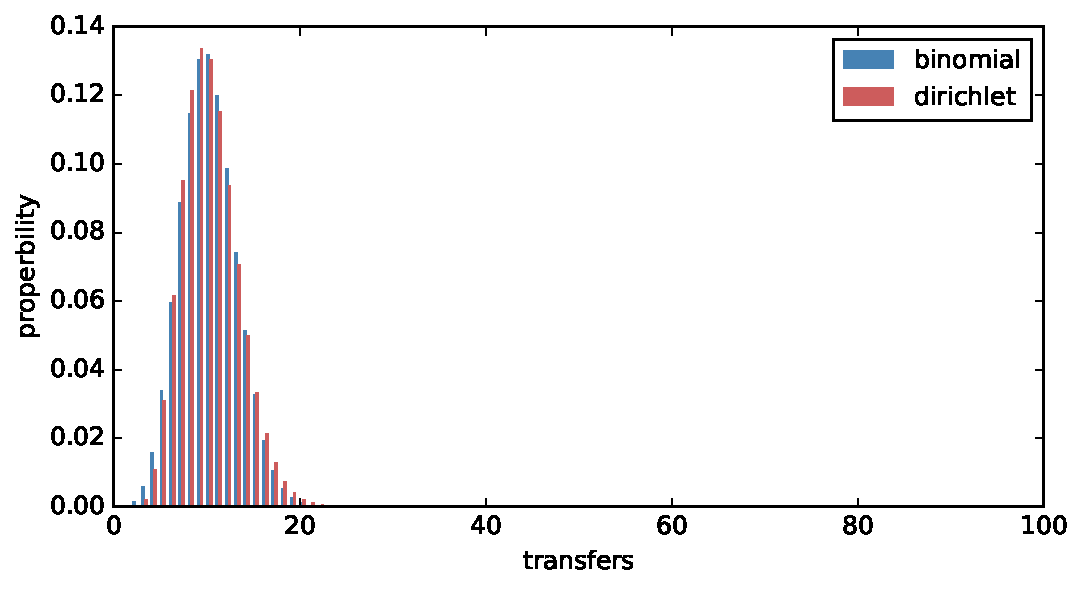
\includegraphics[width= 0.8 \linewidth]{plots/dirichlet-validation-marginal}
	\caption{Comparison of the marginal probability $P(\iround*{N X_1})$ with the binomial distribution. The Dirichlet distribution was scaled up by $N$, $\tau = (0.1, 0.1)$ and $N = 100$.}
	\label{fig:dirichlet-validation-marginal}
\end{figure}

\begin{figure}[H]
	\centering
	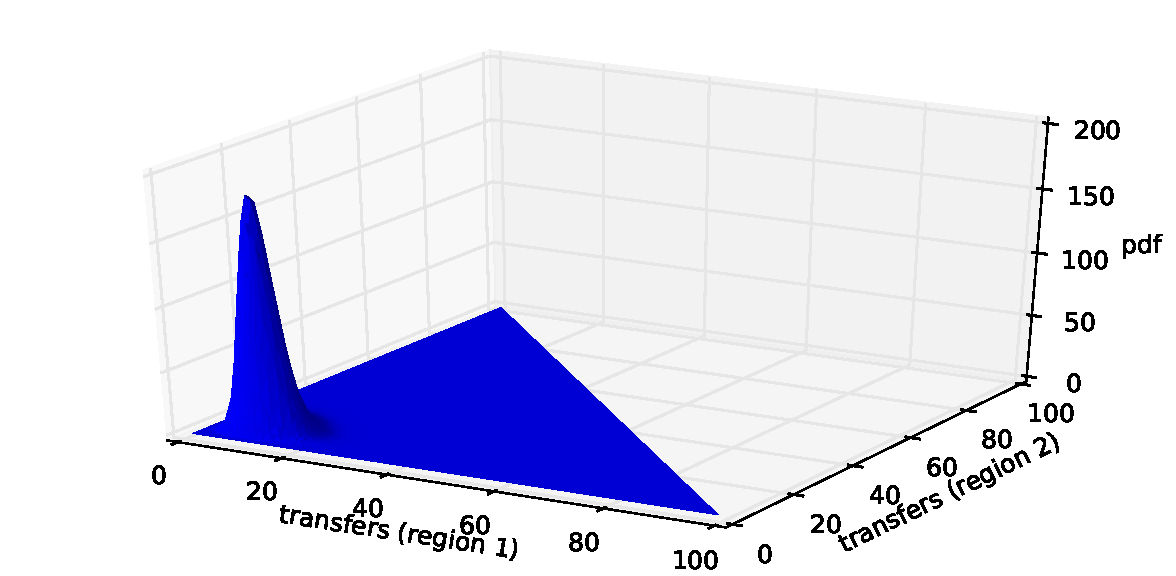
\includegraphics[width= 0.8 \linewidth]{plots/dirichlet-validation-pdf}
	\caption{Shows the Dirichlet pdf with $X_3 = 1- X_1 - X_2$. The Dirichlet distribution is scaled with $N$, $\tau = (0.1, 0.1)$ and $N = 100$.}
\end{figure}

\subsection{Transfer probabilities}

The GLEaM model \cite{GLEaM} uses a gravity law for transferring people between neighboring regions within the same country and airline data for transferring people between airports. Unfortunately the GLEaM paper does not specify all the parameters for the gravity law equation and our airline dataset does not contain the traveling frequency. Instead a much simpler model, where the proportional transfer expectation is fixed to some constant, is used:
\begin{equation}
\sum_{i = 1}^{K_k} \tau_{k, i} = p_{transfer}
\end{equation}

Using an equal transfer probability one gets $\tau_{k, i} = \frac{p_{transfer}}{K_k}$. To ensure that the population doesn't change over time, this value is used to transfer both from $k$ to $i$ and from $i$ to $k$, the equivalent transfer probability of this is:
\begin{equation}
\tau_{k, i} = \frac{p_{transfer}}{K_k} + \frac{p_{transfer}}{K_i} = p_{transfer} \left(\frac{1}{K_k} + \frac{1}{K_i}\right)
\end{equation}

Finally one should be wary of transferring more people to the destination than what is already in the destination. To prevent this the transfer probability is scaled with the relative population.
\begin{equation}
\tau_{k, i} = p_{transfer} \frac{N_i}{N_k + N_i} \left(\frac{1}{K_k} + \frac{1}{K_i}\right)
\end{equation}

Using these transfer probabilities the total population for each region will be unchanged since the transfer expectation is symmetric:
\begin{equation}
\mathbb{E}[N_k \tau_{k, i}] = \mathbb{E}[N_i \tau_{i, k}] \Leftrightarrow N_k \tau_{k, i} = N_i \tau_{i, k}
\end{equation}
